\documentclass{standalone}
\usepackage{tikz}
\usetikzlibrary{positioning,fit,calc,decorations.pathreplacing,arrows,shapes}

\tikzstyle{block} = [draw, rounded corners,rectangle, minimum height=1.8em, minimum width=10em, text centered]
\tikzstyle{arrow} = [thick,->,>=stealth]
\tikzstyle{arrowrev} = [thick,<-,>=stealth]

\begin{document}
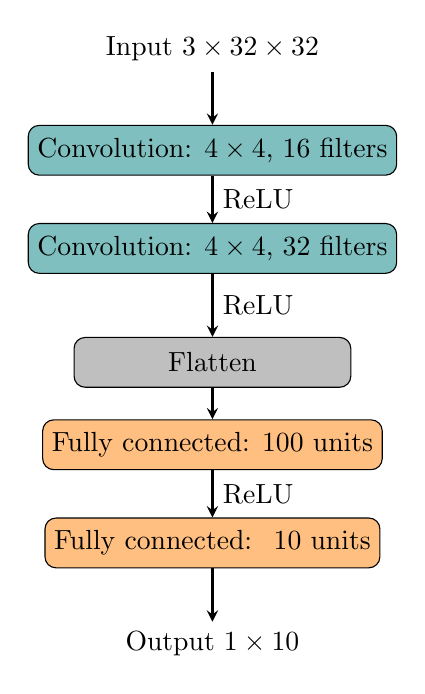
\begin{tikzpicture}

    \node[block, fill=teal!50                    ] (l1) {Convolution: $4\times 4$, 16 filters};
    \node[block, fill=teal!50  , below=.6cm of l1] (l2) {Convolution: $4\times 4$, 32 filters};
    \node[block, fill=gray!50  , below=.8cm of l2] (l3) {Flatten};
    \node[block, fill=orange!50, below=.4cm of l3] (l4) {Fully connected: 100 units};
    \node[block, fill=orange!50, below=.6cm of l4] (l5) {Fully connected: ~10 units};
    
    \draw[arrowrev] (l1) -- ++ (0, 1) node[above] {Input $3\times 32 \times 32$};
    \draw[arrow]    (l5) -- ++ (0,-1) node[below] {Output $1\times 10$};
    \draw[arrow]    (l1) -- (l2) node[midway, right] {ReLU};
    \draw[arrow]    (l2) -- (l3) node[midway, right] {ReLU};
    \draw[arrow]    (l3) -- (l4);
    \draw[arrow]    (l4) -- (l5) node[midway, right] {ReLU};

\end{tikzpicture}
\end{document}